\section{Kupfer-PVD}
\label{copperpvd}

Ein zweites PVD-System stellt Kupfer dar, für das eine Vielzahl an unterschiedlichen Parametrisierungen vorliegt (Tabelle \ref{tab:copperpots}).
Es stellt sich die Aufgabe, darunter eine passende Parametrisierung zu suchen und zu entscheiden, inwiefern eine Vorauswahl anhand weniger Parameter \todo{chword} möglich ist.

\begin{table}[hbtp]
  \caption[EAM-Parametrisierungen für Kupfersysteme]{EAM-Parametrisierungen für Kupfersysteme.}
  \label{tab:copperpots}
  \rowcolors{0}{white}{lightgray}
  \begin{tabularx}{\textwidth}{|lXc|}
    \hline
    \textbf{Bezeichnung} & \textbf{Anwendung \& Kommentare} & \textbf{Ref.} \\
    \hline
    CuAg.eam.alloy & Strukturelle und thermische Eigenschaften von \ce{Cu-Ag} & \cite{williams_embedded-atom_2006} \\
    cu\_ag\_ymwu.eam.alloy & Mono-, Di-, Trimere und Inseln von \ce{Cu} auf \ce{Ag} & \cite{wu_cu/ag_2009} \\
    Cu\_smf7.eam & Oberflächen von \ce{Ni-Cu}-Legierungen bei \SI{800}{\kelvin} & \cite{foiles_calculation_1985} \\
    Cu\_u3.eam & Oberflächen und Bulks verschiedener Legierungen & \cite{foiles_embedded-atom-method_1986} \\
    Cu\_u6.eam & Aktivierungsenergie für Eigendiffusionen & \cite{adams_self-diffusion_1989} \\
    Cu-Zr\_2.eam.fs & Flüssige und amorphe \ce{Cu-Zr}-Legierungen & \cite{mendelev_development_2009} \\
    Cu-Zr.eam.fs & Flüssige und amorphe \ce{Cu-Zr}-Legierungen & \cite{mendelev_using_2007} \\
    Mendelev\_Cu2\_2012.eam.fs & Unterkühlte \ce{Al-Cu}-Schmelzen. Basiert auf \cite{mendelev_analysis_2008} & \cite{_interatomic_2014} \\
    \hline
  \end{tabularx}
  
\end{table}

Viele der Parametersätze wurden für Legierungen angepasst, die Cu-Zr-Potentiale sind sogar mit der Warnung versehen, man könne ein reines Metall damit nicht mehr verlässlich simulieren.
Ein Hinweis auf die Kompatibilität mit LAMMPS oder den untersuchten Systemen ließ sich häufig nicht finden, weshalb Testrechnungen an Kupfer-Bulks und -Oberflächen durchgeführt wurden.

\subsection{Voruntersuchungen}

Mit Ausnahme der drei Parametersätze Cu\_u3.eam, Cu\_u6.eam und Cu\_smf7.eam konnten die Potentiale nicht von LAMMPS zur Simulation genutzt werden.
Es zeigten sich dabei Probleme beim Laden der Dateien, kryptische Fehlerausgaben nach einigen Schritten oder ein Aufhängen der Simulation ohne Vorankündigung.
Die Ergebnisse der verbliebenen Potentiale sind jedoch in guter Übereinstimmung mit Literaturwerten (Tabelle \ref{tab:copperpreresults}).
\todo[inline]{Dichte}
Im Gegensatz zu den ebenfalls durch EAM-Potentiale simulierten Goldsystemen wurde der Schmelzpunkt nicht zuverlässig simuliert (Abbildung \ref{fig:copperthermo}), was durch die sonst geringen Simulationstemperaturen vernachlässigbar ist.

\begin{table}[tbh]
  \rowcolors{0}{white}{lightgray} 
  \caption[Eigenschaften von Kupfer]{Vergleich der Eigenschaften von Kupfer mit experimentellen und Literaturdaten als Voruntersuchung des PVD-Prozesses\todo[inline]{ref}}
  \label{tab:copperpreresults}
  \begin{tabularx}{\textwidth}{|lXXXX|}
    \hline
    \textbf{unters. Größe} & \textbf{Experiment} & \textbf{Cu\_smf7.eam} & \textbf{Cu\_u3.eam} & \textbf{Cu\_u6.eam} \\
    \hline
    Koordination   &  \SI{12.00}{} & \SI{12.00}{} & \SI{12.00}{} & \SI{12.00}{} \\
    Bindungslänge  &  \SI{2.556}{\angstrom} & \SI{2.558}{\angstrom} (\SI{0.08}{\percent}) & \SI{2.558}{\angstrom} (\SI{0.08}{\percent}) & \SI{2.558}{\angstrom} (\SI{0.08}{\percent}) \\
    Dichte         & \SI{8.92}{\gram\per\cubic\centi\meter} & \SI{8.908}{\gram\per\cubic\centi\meter} (\SI{-0.13}{\percent}) & \SI{8.915}{\gram\per\cubic\centi\meter} (\SI{-0.06}{\percent}) & \SI{8.910}{\gram\per\cubic\centi\meter}  (\SI{-0.11}{\percent}) \\
    \hline
  \end{tabularx}
\end{table}

\todo[inline]{Oberflächenvalidierung?}

\begin{figure}[bht]
  \captionsetup[subfigure]{singlelinecheck=false}
  \def\subfigwidth{7cm}
  \begin{subfigure}[t]{\subfigwidth}
    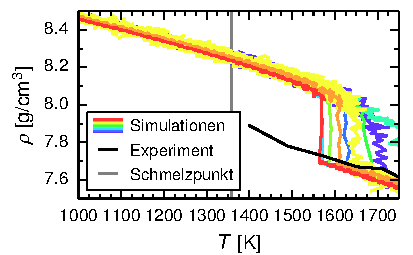
\includegraphics[width=\textwidth]{Cu_u6_meltingpoint}
    \subcaption{Phasenübergang mit Cu\_u6.eam bei unterschiedlichen $t_\text{relax}$}
  \end{subfigure}
  \hfill
  \begin{subfigure}[t]{\subfigwidth}
    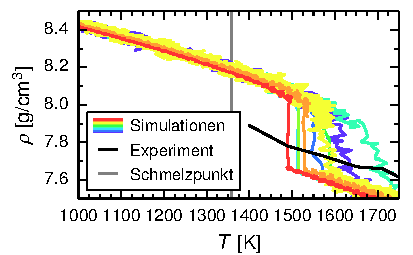
\includegraphics[width=\textwidth]{Cu_smf7_meltingpoint}
    \subcaption{Phasenübergang mit Cu\_smf7.eam bei unterschiedlichen $t_\text{relax}$}
  \end{subfigure}
  \caption[Abweichung der Schmelztemperaturen bei Kupfer-MD]{
    Abweichung der Schmelztemperatur mit verschiedenen Parametrisierungen.
    Experimentelle Werte von Brillo et al.\cite{brillo_density_2006}.
  }
  \label{fig:copperthermo}
\end{figure}

\subsection{Prozess-Simulation}

Aufgrund der Ähnlichkeit des Gold-PVD-Prozesses wurden dessen Parameter für die Kupfer-PVD übernommen und auf dessen Eigenschaften leicht angewandt.
So liegen kleinere Bindungslängen und geringere Massen vor, die beispielsweise zu erhöhten \todo{wirklich?}Auftreffgeschwindigkeiten führen.

Zu Beginn der Simulation ergeben sich hohe Abbruchquoten von \SI{25}{\percent}, die im Laufe der Simulation nachlassen.
Genauere Untersuchungen zeigen, dass bei Ankunft eines neuen Kupferatomes auf der glatten Gitteroberfläche ein vorhandenes Atom herausgeschlagen wird.
Sobald die Oberfläche mit genügend Off-Lattice-Atomen versehen ist, verschwindet dieser Effekt.
Die kritische Bedeckung liegt zwischen \SI{0.034}{\per\nano\meter\squared} und \SI{0.074}{\per\nano\meter\squared}, was sich mit der maximalen MD-Ereignisdichte von \SI{0.073}{\per\nano\meter\squared} deckt.
Es ist also zu vermuten, dass perfekte Gitterkonfigurationen nicht robust gegenüber gerichteten Energieeinträgen ist, kleine Perturbationen der Atompositionen aber zur gleichmäßigeren Verteilung der eingebrachten Energien führen.
\todo[inline]{Entropie?}

\begin{figure}[bth]
  \captionsetup[subfigure]{singlelinecheck=false}
  \def\subfigwidth{0.49\textwidth}
  \begin{subfigure}[t]{\subfigwidth}
    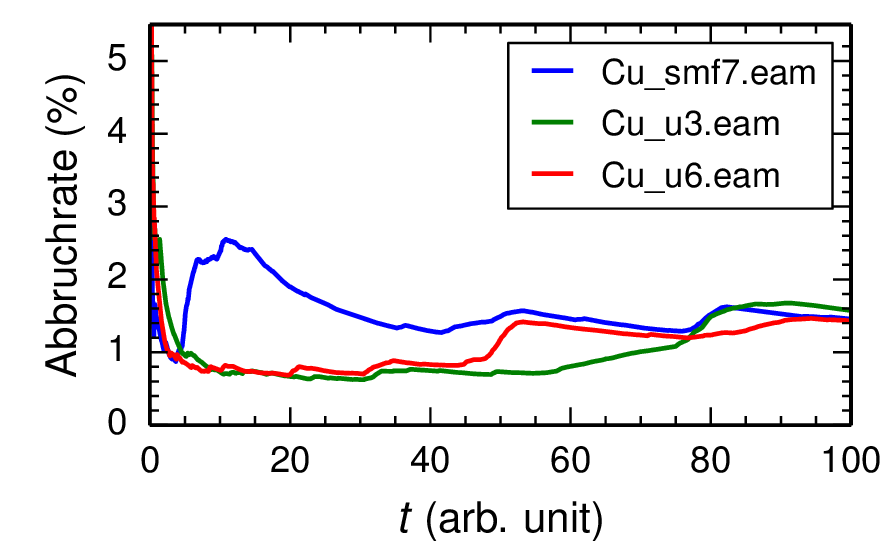
\includegraphics[width=\textwidth]{Cu_abortstatplot}
    \subcaption{Verlauf der Abbruchraten}
    \label{fig:copperparsivald-a}
  \end{subfigure}
  \hfill
  \begin{subfigure}[t]{\subfigwidth}
    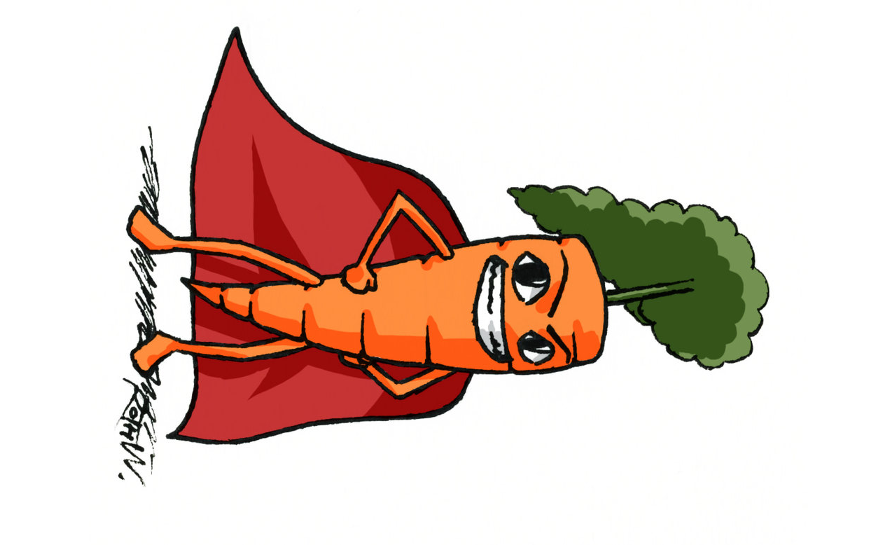
\includegraphics[width=\textwidth]{missing}
    \subcaption{Zeitliche Entwicklung der Schichtdicke}
    \label{fig:copperparsivald-b}
  \end{subfigure}
  \begin{subfigure}[t]{\subfigwidth}
    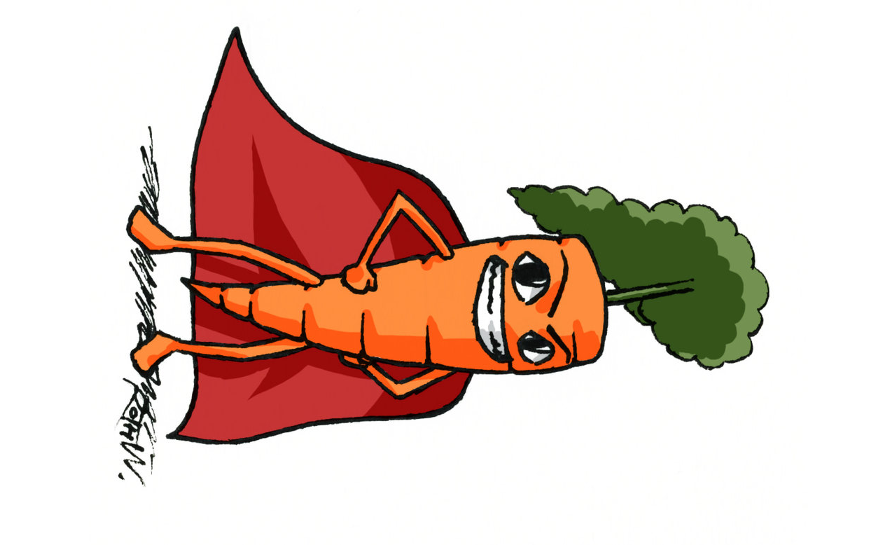
\includegraphics[width=\textwidth]{missing}
    \subcaption{Zeitliche Entwicklung der Rauheit}
    \label{fig:copperparsivald-c}
  \end{subfigure}
  \hfill
  \begin{subfigure}[t]{\subfigwidth}
    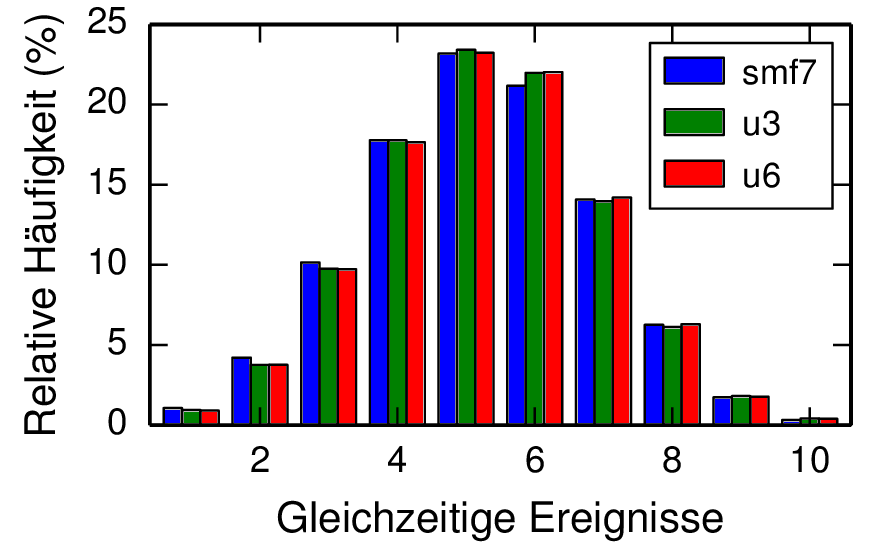
\includegraphics[width=\textwidth]{Cu_eventhistogram}
    \subcaption{Häufigkeit gleichzeitiger Ereignisse}
    \label{fig:copperparsivald-d}
  \end{subfigure}
  \caption{Vergleich der Kupfer-Potentiale im Parsivald-Programm}
  \label{fig:copperparsivald}
\end{figure}

Im weiteren Verlauf der Simulation konvergiert die Abbruchquote gegen einen niedrigen Wert unterhalb von \SI{2}{\percent} (Abbildung \ref{fig:copperparsivald-a}).
Strukturelle Untersuchungen zeigen keine Einschlüsse, was auch bei diesem Prozess durch in der fcc-kristallinen Struktur der abgeschiedenen Schicht begründet ist.
Rauheit und Schichtdicke (Abbildungen \ref{fig:copperparsivald-b} und \ref{fig:copperparsivald-c}) \todo{SCHÖNER!}{sind schön}.

\subsubsection{Maximale Ereignisdichte}
Ergänzend ist in Abbildung \ref{fig:copperparsivald-d} ein Histogramm der Zahl paralleler Ereignisse dargestellt.
Die maximale Oberflächendichte der Ereignisse liegt bei der gewählten MD-Box-Größe von \SI{37x37}{\angstrom} bei \SI{0.073}{\per\nano\meter\squared}.
Dem stehen beobachtete Werte von 12 aktiven Ereignissen gegenüber, die einer Dichte von \SI{0.03}{\per\nano\meter\squared} und somit \SI{30}{\percent} maximaler Bedeckung entsprechen.
Aufgrund der zufälligen Positionierung der MD-Box innerhalb der KMC-Simulation und der Blocking von Ereignissen bei Überlappung der MD-Kästen scheint dieser Wert plausibel.
Ähnliche Werte werden bei Simulationsläufen mit unterschiedlichen Substratgrößen und Materialien beobachtet werden.
